\subsection{Introduction} \label{subsect:case-study:intro}

This section describes the overall idea of the case study and how it was used to examine the \mlblink algorithm.

\subsubsection{User Interface} \label{subsubsect:case-study:intro:ui}
% Introduction to Case Study
The case study consists of a user interface (UI) that allows users to match two images of the same location in the night sky from distinct datasets, and an Application Programming Interface (API) that processes data created by the UI. Figure \ref{fig:ml-blink-ui-main-screen} shows the UI where users can create a matching of two images. Through out the report, an arrangement of two images from the same location of the night sky from distinct datasets is described as a mission.

\begin{figure}[H]
  \centering
  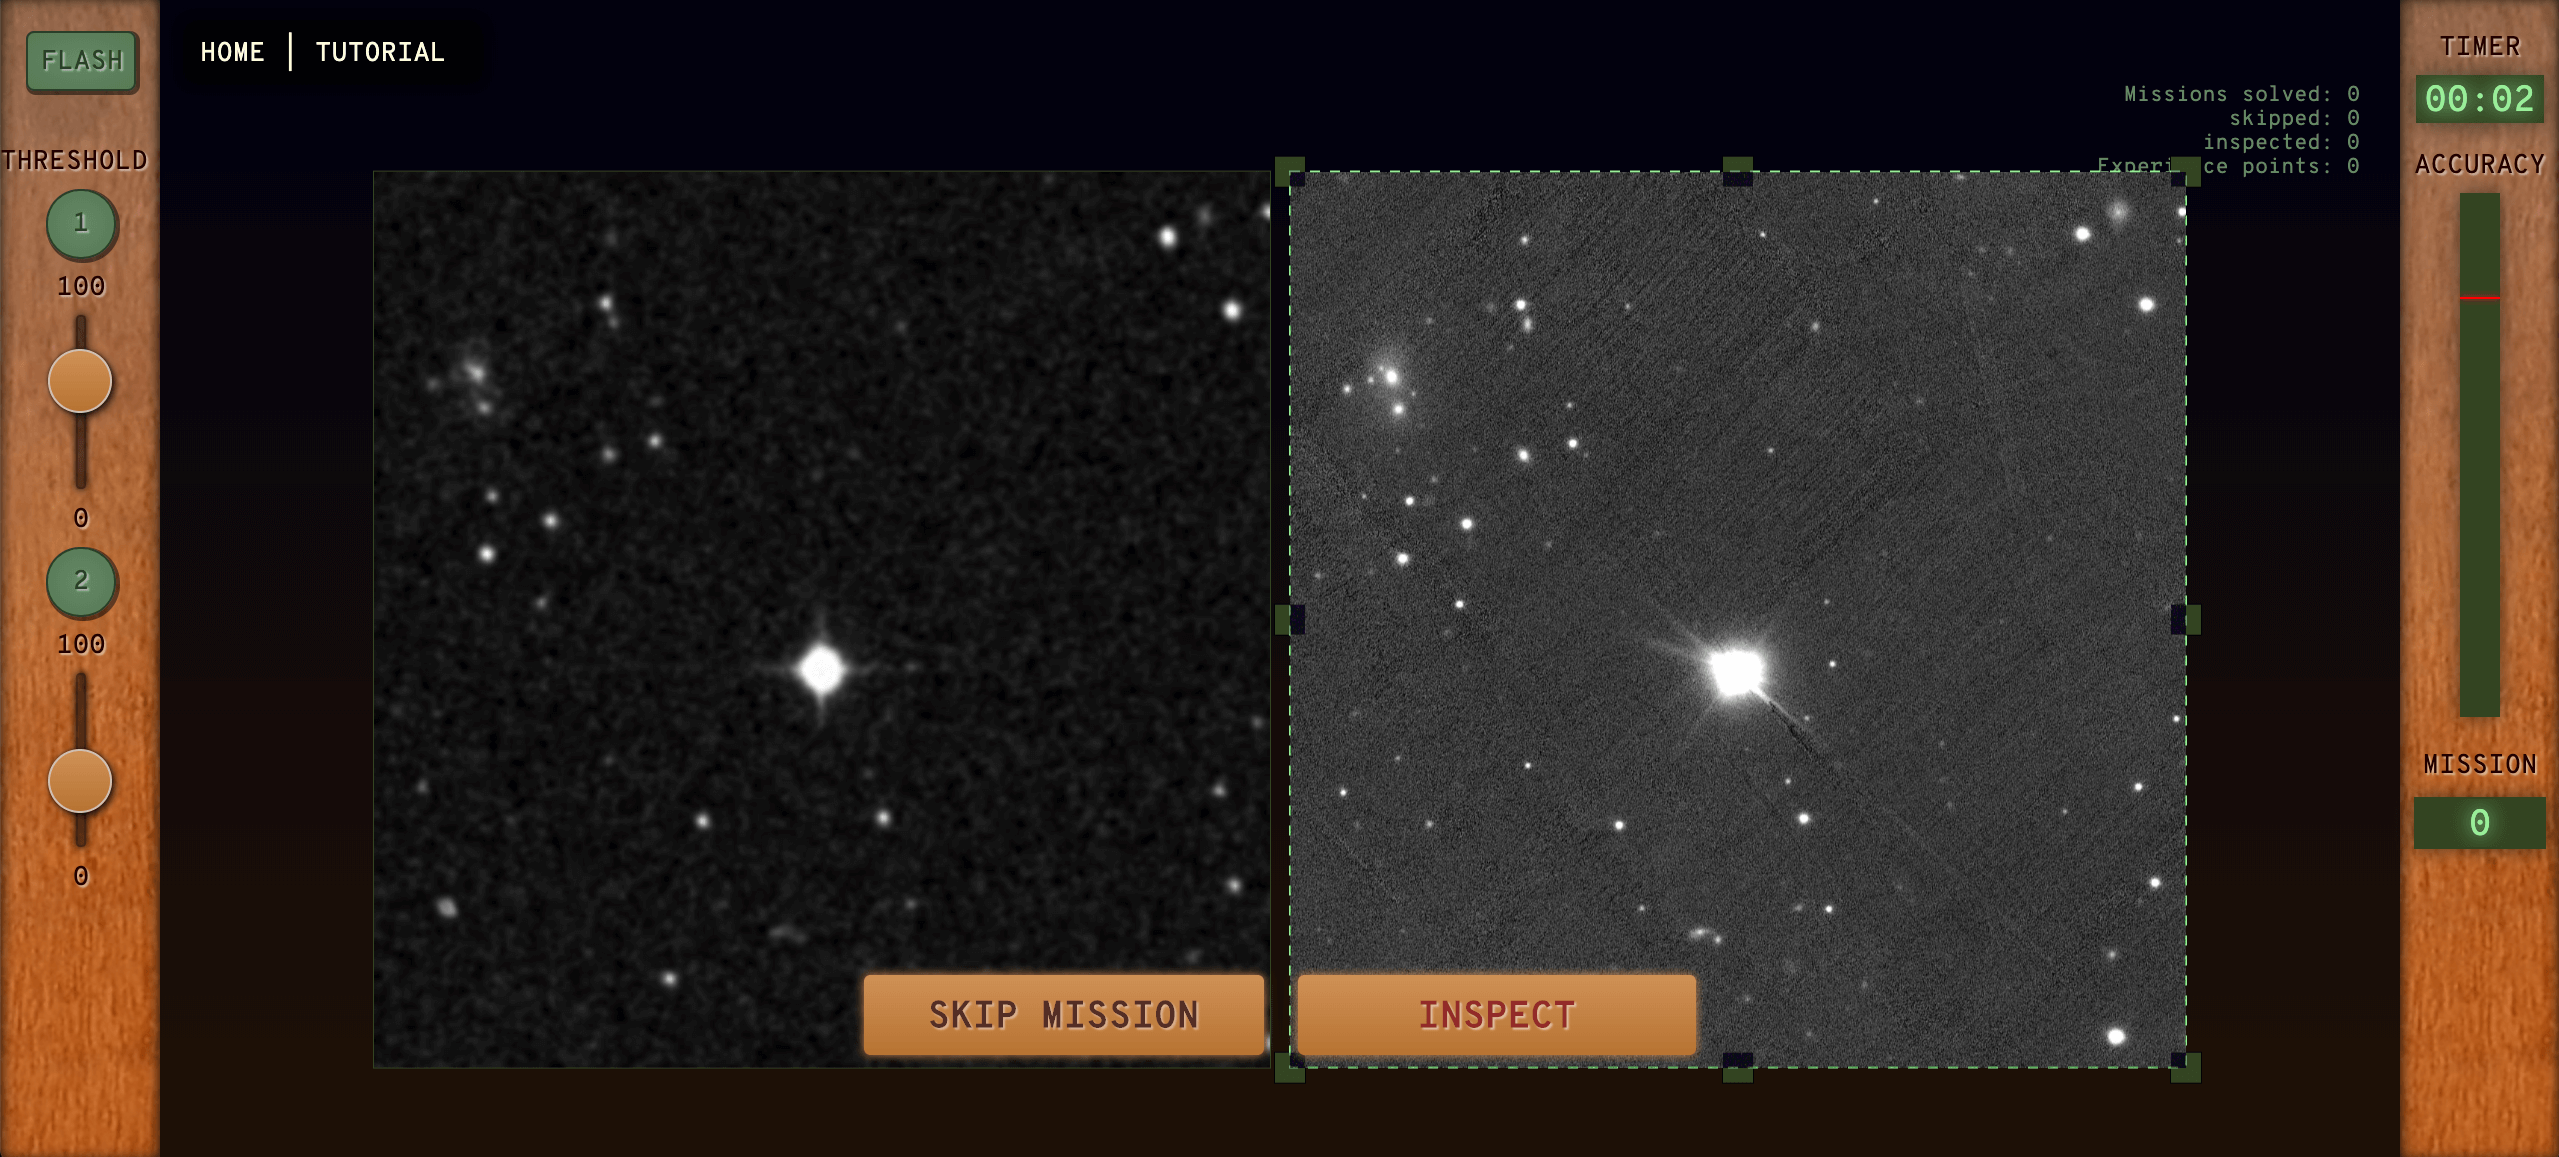
\includegraphics[
        width=\textwidth,
        height=\textheight,
        keepaspectratio
  ]{report/images/ml-blink-ui-main-screen.png}
  \caption{UI used to conduct the case study. Users are presented a mission where the goal is to create a matching. A matching is defined as the placing of the right side image on top of the other one, and obtaining an accuracy based on how good such matching is (i.e. how well the objects of one image align with the objects of the other image). The accuracy achieved by a matching is shown to the user in the right side of the UI.}
  \label{fig:ml-blink-ui-main-screen}
\end{figure}

\subsubsection{Datasets} \label{subsubsect:case-study:intro:datasets}

% What is USNO-B1.0?
\todo[inline]{TODO: What is Pan-STARRS1?}
The case study was carried out using a subset of the \usno and \panstarrs datasets. \usno is an all-sky catalog composed from multiple sky surveys during the interval from 1949 to 2002 \cite{web:caltech:usno} that indicates positions, proper motions, star/galaxy estimators and other astronomical features for 1,042,618,261 objects derived from 3,643,201,733 distinct observations \cite{web:ap-i:usno}. \panstarrs in the other hand, is a [...].

The subset consisted of a total of 1000 unique cases in each dataset, each described across different bands. The \usno subset used a total of five bands (\texttt{blue1}, \texttt{blue2}, \texttt{red1}, \texttt{red2}, and \texttt{ir}), while \panstarrs used a total of three bands (\texttt{g}, \texttt{r}, and \texttt{z}). Table \ref{table:case-study:intro:datasets-mapping} shows how each of these bands are related to one another in \usno and \panstarrs.

\begin{table}[H]
    \centering
        \begin{tabular}{| c | c |} 
            \hline
                \usno Band & \panstarrs Band \\
            \hline
                \texttt{blue1} & \texttt{g} \\
            \hline
                \texttt{blue2} & \texttt{g} \\
            \hline
                \texttt{red1} & \texttt{r} \\
            \hline
                \texttt{red2} & \texttt{r} \\
            \hline
                \texttt{ir} & \texttt{z} \\
            \hline
        \end{tabular}
    \caption{Mappings which specify how each band in \usno is related to a band in \panstarrs or vice--versa.}
    \label{table:case-study:intro:datasets-mapping}
\end{table}

\subsubsection{Matching Accuracy} \label{subsubsect:case-study:intro:matching-accuracy}
The UI uses an accuracy threshold shown to the user in the right side of the screen to determine whether a matching of two images is good or not. If a user is able to achieve an accuracy greater or equal than that of the accuracy threshold, the mission is then considered to be successfully completed and the two images are unlikely to contain an anomaly. If the accuracy achieved by the user is less than that of the accuracy threshold, then the images that represent the mission are considered to be potential anomalies. 

The accuracy threshold used to conduct the case study was fixed at $80$\%. To fix it, a few missions from the datasets were randomly selected and manually altered to represent anomalies of interest, such as replacing a bright section of one of the images with its background, while the other image remained unaltered. Figure \ref{fig:fake:mission-13} shows an example of an anomaly that was manually created, where the center object of the image from the \panstarrs dataset has been replaced by its background. When missions like this were presented in the UI, it was found to be difficult, and in some occasions impossible, to get an accuracy greater than $80$\%, and thus why it was selected as the accuracy threshold.

\begin{figure}[H]
    \centering
    \begin{subfigure}{.5\textwidth}
      \centering
      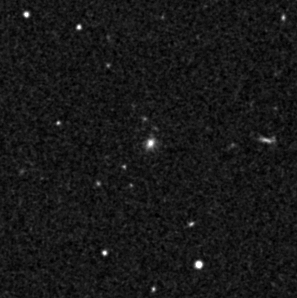
\includegraphics[
            width=\textwidth,
            height=0.30\textheight,
            keepaspectratio
        ]{report/images/fake-anomalies/usno-13-blue1.png}
      \caption{\usno}
      \label{fig:a:fake:usno-13-blue1}
    \end{subfigure}%
    \begin{subfigure}{.5\textwidth}
      \centering
      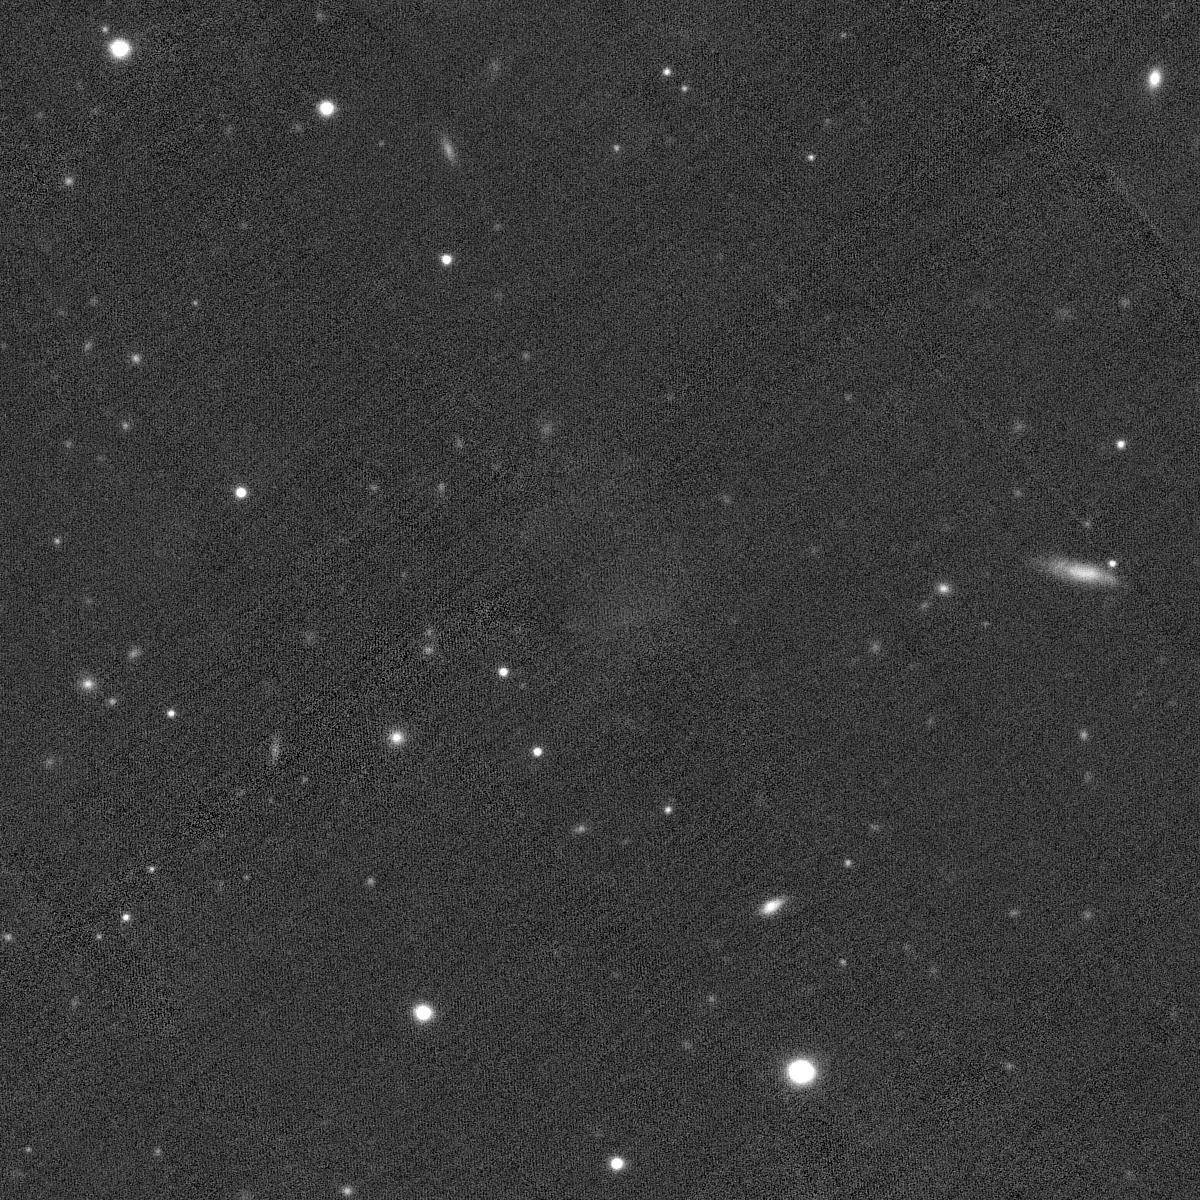
\includegraphics[
            width=\textwidth,
            height=0.30\textheight,
            keepaspectratio
      ]{report/images/fake-anomalies/panstarr-13-g.png}
      \caption{\panstarrs}
      \label{fig:b:fake:panstarr-13-g}
    \end{subfigure}
    \caption{Figures \ref{fig:a:fake:usno-13-blue1} and \ref{fig:b:fake:panstarr-13-g} show pictures manually altered taken from the same location in the night sky from \usno and \panstarrs respectively. An object in the center of the \panstarrs image has been replaced by the image's background, while the \usno image is unaltered.}
    \label{fig:fake:mission-13}
\end{figure}

% > Overall idea of the case study